\section{Ejercicio 1}

\subsection{Introducción}

En este ejercicio se plantea una máquina de estados para controlar la carga de un tanque de agua mediante la utilización de dos bombas independientes. \par
La cátedra solicita una implementación mediante una máquina de Moore, la cual se caracteriza porque las salidas no dependan de las entradas. Estas últimas servirán para realizar cambios de estado y controlar el flujo general de la máquina. Por otro lado, cada estado tendrá asociado una salida. La implementación característica de una máquina de Moore se presenta a continuación:

\begin{figure}[H]
\begin{center}
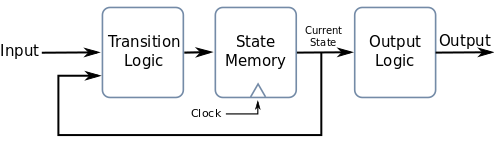
\includegraphics[scale=0.8]{Ejercicio1/Imagenes/moore}
\caption{Máquina de Moore}
\end{center}
\label{Maquina_de_Moore}
\end{figure}

Los sensores $S$ e $I$ ubicados en la parte superior e inferior del tanque respectivamente, actuarán como las entradas de la máquina de estado, su valor será $1$ al detectar agua y $0$ en caso contrario. Para la implementación se utilizarán cuatro estados los cuales indicarán el estado de funcionamiento de las bombas como se muestra en la tabla (\ref{Estados_utilizados}). \par
Para representar dichos estados son necesarios dos bits, como dichos bits representarán el estado de las bombas, los estados coincidirán con las salidas de la máquina de Moore.
 

\begin{table}[H]
	\begin{center}
	\scalebox{0.9}{
		\begin{tabular}{c|c|c}
		Estado & $Q_1$                  & $Q_0$ \\ \hline
		A      & \multicolumn{1}{c|}{0} & 0     \\
		B      & \multicolumn{1}{c|}{0} & 1     \\
		C      & \multicolumn{1}{c|}{1} & 0     \\
		D      & \multicolumn{1}{c|}{1} & 1    
		\end{tabular}
	}
	\caption{Estados utilizados}
	\label{Estados_utilizados}
	\end{center}

\end{table}


 Donde dichos estados representan:\newline 
 A: Ninguna bomba está encendida \newline
 B: La bomba 0 está encendida \newline
 C: La bomba 1 está encendida \newline
 D: Ambas bombas están encendidas \newline
 \par
 
\subsection{Tabla de transiciones y diagrama de estados}

Todas las transiciones posibles se pueden observar en el tabla (\ref{Transiciones_Ej1}). Se plantean las siguientes consideraciones:

\begin{itemize}
	\item Si llega la entrada I=0 y S=1, lo que implicaría que se detecta agua en la parte superior pero no en la inferior, se considera un absurdo y la máquina se mantendrá en su estado actual.
	\item Para la transición entre los estados A y D a los estados B o C, con esta tabla resulta imposible determinar cuál fue la última bomba encendida por lo que se pondrá "Don't care". Para realizar dichas transiciones se realizará una lógica aparte.

\end{itemize}

\begin{table}[H]
\begin{center}
\scalebox{0.8}{
\begin{tabular}{c|cc|cc|c|cc}
$E$ & $Q_1$                  & $Q_0$ & $I$                    & $S$ & $E^*$ & ${Q_1}^*$                 & ${Q_0}^*$ \\ \hline
A   & \multicolumn{1}{c|}{0} & 0     & \multicolumn{1}{c|}{0} & 0   & D    & \multicolumn{1}{c|}{1} & 1      \\
A   & \multicolumn{1}{c|}{0} & 0     & \multicolumn{1}{c|}{0} & 1   & A    & \multicolumn{1}{c|}{0} & 0      \\
A   & \multicolumn{1}{c|}{0} & 0     & \multicolumn{1}{c|}{1} & 0   & X    & \multicolumn{1}{c|}{X} & X      \\
A   & \multicolumn{1}{c|}{0} & 0     & \multicolumn{1}{c|}{1} & 1   & A    & \multicolumn{1}{c|}{0} & 0      \\
B   & \multicolumn{1}{c|}{0} & 1     & \multicolumn{1}{c|}{0} & 0   & D    & \multicolumn{1}{c|}{1} & 1      \\
B   & \multicolumn{1}{c|}{0} & 1     & \multicolumn{1}{c|}{0} & 1   & B    & \multicolumn{1}{c|}{0} & 1      \\
B   & \multicolumn{1}{c|}{0} & 1     & \multicolumn{1}{c|}{1} & 0   & B    & \multicolumn{1}{c|}{0} & 1      \\
B   & \multicolumn{1}{c|}{0} & 1     & \multicolumn{1}{c|}{1} & 1   & A    & \multicolumn{1}{c|}{0} & 0      \\
C   & \multicolumn{1}{c|}{1} & 0     & \multicolumn{1}{c|}{0} & 0   & D    & \multicolumn{1}{c|}{1} & 1      \\
C   & \multicolumn{1}{c|}{1} & 0     & \multicolumn{1}{c|}{0} & 1   & C    & \multicolumn{1}{c|}{1} & 0      \\
C   & \multicolumn{1}{c|}{1} & 0     & \multicolumn{1}{c|}{1} & 0   & C    & \multicolumn{1}{c|}{1} & 0      \\
C   & \multicolumn{1}{c|}{1} & 0     & \multicolumn{1}{c|}{1} & 1   & A    & \multicolumn{1}{c|}{0} & 0      \\
D   & \multicolumn{1}{c|}{1} & 1     & \multicolumn{1}{c|}{0} & 0   & D    & \multicolumn{1}{c|}{1} & 1      \\
D   & \multicolumn{1}{c|}{1} & 1     & \multicolumn{1}{c|}{0} & 1   & D    & \multicolumn{1}{c|}{1} & 1      \\
D   & \multicolumn{1}{c|}{1} & 1     & \multicolumn{1}{c|}{1} & 0   & X    & \multicolumn{1}{c|}{X} & X      \\
D   & \multicolumn{1}{c|}{1} & 1     & \multicolumn{1}{c|}{1} & 1   & A    & \multicolumn{1}{c|}{0} & 0     
\end{tabular}}
\caption{Transiciones entre estados}
\label{Transiciones_Ej1}
\end{center}
\end{table}

La tabla anterior nos indicará la lógica de entrada para un Caso I mientras que para transiciones entre los estados A y D a los estados B o C se considerará la lógica para un Caso II.


A continuación, se representa el diagrama de estados y la tabla de transiciones resumida de nuestra máquina para el Caso I.
 

\begin{table}[H]
\begin{center}
\scalebox{0.7}{
\begin{tabular}{c|cc|cc}
\multirow{2}{*}{\begin{tabular}[c]{@{}c@{}}Estado \\ Actual\end{tabular}} & \multicolumn{2}{c|}{S=0}     & \multicolumn{2}{c}{S=1}     \\
                                                                          & I=0                    & I=1 & I=0                    & I=1 \\ \hline
A                                                                         & \multicolumn{1}{c|}{D} & A   & \multicolumn{1}{c|}{X} & A   \\
B                                                                         & \multicolumn{1}{c|}{D} & B   & \multicolumn{1}{c|}{B} & A   \\
C                                                                         & \multicolumn{1}{c|}{D} & C   & \multicolumn{1}{c|}{C} & A   \\
D                                                                         & \multicolumn{1}{c|}{D} & D   & \multicolumn{1}{c|}{X} & A	\\
\end{tabular}
}
\label{Tabla_de_transiciones_Ej1}
\caption{Tabla de transiciones}
\end{center}
\end{table}

 \begin{figure}[H]
\begin{center}
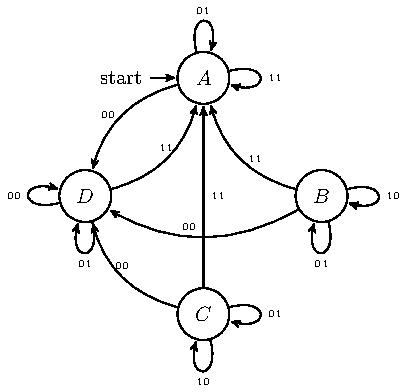
\includegraphics[scale=0.9]{Ejercicio1/Diagramas/Transiciones}
\caption{Diagrama de estados}
\end{center}
\label{Diagrama_de_estados_Ej1}
\end{figure}

\subsection{Implementación - Caso I}

Se necesitan dos bits para almacenar los cuatro estados utilizados, por lo que se necesitarán dos Flip-Flop D para guardarlos en memoria.
Desarrollando las tablas obtenemos los siguientes mapas de Karnaugh que nos indicarán los circuitos lógicos necesarios para el Caso I.

%Mapas de Karnaugh 
\begin{center}
	\hspace*{\fill}
   \begin{tikzpicture}[x=1cm,y=1cm]
    \K[x bits = 2, y bits = 2, label={$Y_1$},
       variable names = {$I$,$S$,$Q_1$,$Q_0$,}]
    { 
      0000,1,    
      0001,1,   
      0010,1,   
      0011,1,       
      0100,0, 
      0101,0,
      0110,1,
 	  0111,1,
 	  1000,X,    
      1001,0,   
      1010,1,   
      1011,X,       
      1100,0, 
      1101,0,
      1110,0,
 	  1111,0,
    }
    \newcommand*{\myKG}[4][0.1]{\KG[x bits = 2,y bits = 2,group opacity = #1,
                  #2]{#3}{#4}}
    \myKG     {group color = red,  group distance=0.35}{0010}{0000}
    \myKG     {group color = pink,  group distance=0.35}{0010}{0111}
    \myKG     {group color = purple,  group distance=0.35}{1010}{0011}


    %=====================================================================
    % in picture comments
    %=====================================================================

    \path (1,-3.5) node[anchor = north, align = left] (eq1){%
    $D_1 = 
       \ul{red}{$\ol{I}\,\ol{S}\,$}
       +\ul{pink}{${Q_1}\,\ol{I}\,$}  
       +\ul{purple}{${Q_1}\,\ol{S}\,$}  
    $};
    
  \end{tikzpicture}
	\hspace{2mm}
   \begin{tikzpicture}[x=1cm,y=1cm]
    \K[x bits = 2, y bits = 2, label={$Y_1$},
       variable names = {$I$,$S$,$Q_1$,$Q_0$,}]
    { 
      0000,1,    
      0001,1,   
      0010,1,   
      0011,1,       
      0100,0, 
      0101,1,
      0110,0,
 	  0111,1,
 	  1000,X,    
      1001,1,   
      1010,0,   
      1011,X,       
      1100,0, 
      1101,0,
      1110,0,
 	  1111,0,
    }
    \newcommand*{\myKG}[4][0.1]{\KG[x bits = 2,y bits = 2,group opacity = #1,
                  #2]{#3}{#4}}
    \myKG     {group color = red,  group distance=0.35}{0010}{0000}
    \myKG     {group color = pink,  group distance=0.35}{0011}{0101}
    \myKG     {group color = purple,  group distance=0.35}{1011}{0001}


    %=====================================================================
    % in picture comments
    %=====================================================================

    \path (1,-3.5) node[anchor = north, align = left] (eq1){%
    $D_1 = 
       \ul{red}{$\ol{I}\,\ol{S}\,$}
       +\ul{pink}{${Q_1}\,\ol{I}\,$}  
       +\ul{purple}{${Q_1}\,\ol{S}\,$}  
    $};
    
  \end{tikzpicture}
	\hspace{2mm}
	\hspace*{\fill}
\end{center}

Dando como resultado el siguiente circuito:

\begin{figure}[H]
\begin{center}
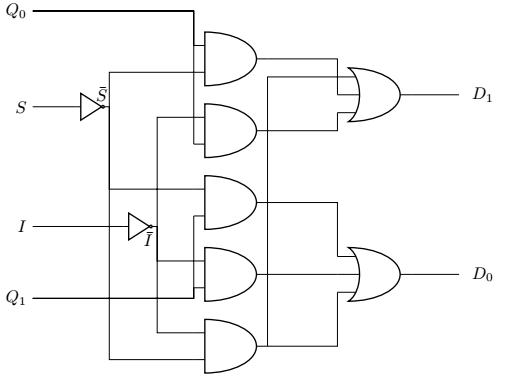
\includegraphics[,scale=0.5]{Ejercicio1/Circuitos/Logica1}
\caption{Lógica de la entrada - Caso I}
\end{center}
\label{Transiciones_Caso_I}
\end{figure}

\subsection{Implementación - Caso II}

Por otro lado, para el Caso II era necesario almacenar cual había sido la última bomba en no activarse por lo que decidió guardar dicha información en un Flip-Flop T. Dicho bit sólo debería ser cambiado bajo dos condiciones, cuando la máquina tenga entradas $I=1$ y $S=0$ estando en el estado A o D. \par Para el primer caso implica que ambas bombas están apagadas y se detecta que el tanque se encuentra por la mitad, por lo que hay que proceeder a activar la última bomba en no activarse. Para el otro, se está trabajando con ambas bombas y se detecta que el reservorio está por la mitad, por lo que se procederá a apagar la última en entrar en servicio.
Las salidas del Flip-Flop T representarán el próximo estado ya que representan el estado de las bombas. \par
El siguiente circuito(\ref{Transiciones_Caso_II}) representa dicha lógica.

\begin{figure}[H]
\begin{center}
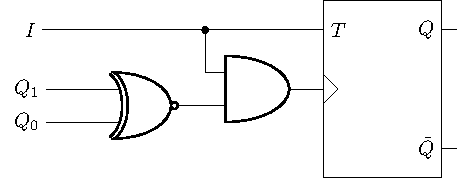
\includegraphics[scale=1]{Ejercicio1/Circuitos/Logica2}
\caption{Lógica de la entrada - Caso II}
\end{center}
\label{Transiciones_Caso_II}
\end{figure}

La entrada $I$ funcionará como el clock del FFT asociado a una compuerta AND que sólo se activará al estar en los estados previamente mencionados. Consecuentemente, el flanco de clock para dicho Flip-Flop sólo llegará al transicionar entre dichos estados.

\subsection{Conexión Caso I y II}

Para finalizar era necesario un circuito que indicará cuando el siguiente estado iba a provenir del cirucito de entrada lógico del Caso I o del Caso II. Por ende, se implementa un multiplexor cuya entrada de activación va a estar dada por el Caso II. \par
Por lo tanto, cuando la variable de control del multiplexor sea 1, el próximo estado va a estar determinado por las salidas del Flip-Flop T mientras que, para el caso contrario, será provisto por el circuito lógico de entrada del Caso I.

\begin{figure}[H]
\begin{center}
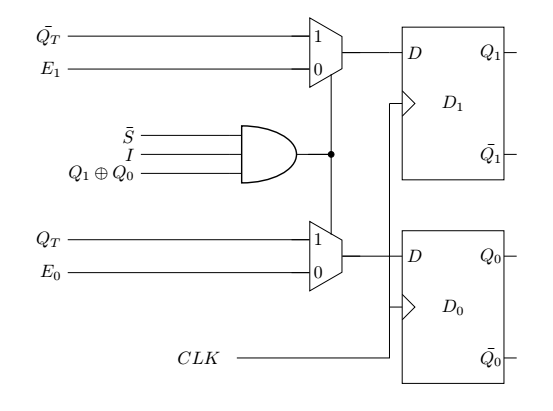
\includegraphics[,scale=0.5]{Ejercicio1/Circuitos/Sumalogica}
\caption{Conexión lógica de las lógicas de entrada}
\end{center}
\label{Logica_entrada_Ej1}
\end{figure}

Se adjunta simulación en Proteus y Verilog para respaldar el diseño.
